%%% CHEP 2019 protoDUNE-SP DQM evolution paper

%%%\documentclass[option]{webofc}
%%% "twocolumn" for typesetting an article in two columns format (default one column)


\documentclass{webofc}
\usepackage[varg]{txfonts}   % Web of Conferences font

%
% Put here some packages required or/and some personnal commands
%

\usepackage{xspace}
\usepackage{tabularx}

\newcommand{\pd}{protoDUNE\xspace}
\newcommand{\filesize}{8\,GB\xspace}

%%%%%%%%%%%%%%%%%%%%%%%%%%%% BEGIN %%%%%%%%%%%%%%%%%%%%%%%%%%%%%%%

\begin{document}
%
\title{Evolution of the Data Quality Monitoring and Prompt Processing System in the protoDUNE-SP experiment}


\author{
\firstname{Maxim} 
\lastname{Potekhin}\inst{1}\fnsep\thanks{\email{potekhin@bnl.gov}}, \it{on behalf of the DUNE Collaboration}
}

\institute{Brookhaven National Laboratory, Upton, NY11973, USA}


\abstract{
The DUNE Collaboration currently operates
an experimental program based at CERN which includes a beam test and an extended
cosmic ray run of two large-scale prototypes of the massive Liquid Argon Time
Projection Chamber for the DUNE Far Detector. The volume of data collected by the single-phase prototype
(protoDUNE-SP) amounts to $\sim$3PB and the sustained rate
of data sent to mass storage is O(100) MB/s.  Data Quality Monitoring
was implemented by directing a fraction of the data stream
to the protoDUNE Prompt Processing System (p3s) which is optimized
for continuous low-latency calculation of the vital detector metrics and various graphics
including event displays. It served a crucial role throughout the life cycle of the
experiment. We present our experience in leveraging the CERN computing
environment and operating the system over an extended period of time, while
adapting to evolving requirements and computing platform.
}
%
\maketitle
%
\section{Introduction}
\label{sec:intro}

The aim of the \pd-SP experiment  \cite{spanu} is a detailed study of a large-scale prototype
of the massive 10kt single-phase Liquid Argon Time Projection Chamber (LArTPC) to be used
in the DUNE experiment  \cite{cdrVol1, cdrVol4}. The experiment took test beam data in
2018 and cosmic ray data throughout 2019. The nature of the experiment requires a versatile
Data Quality Monitoring (DQM) system capable of performing complex calculations on
a few minutes time scale as well as preserving the results (inluding various types of graphics
and tabulated data) in an easily accessible form and over an extended period of time.
In order to support this capability a \textit{prompt processing system} was designed, deployed
and operated for 3 years \cite{eps}. Its design proved flexible enough to quickly adapt to
different hardware platforms and computational payloads.

\section{Outline of the System Design}
\label{sec:outline}

The following is a summary  of the \pd-SP DQM system  design features\cite{chep18}:
\begin{itemize}

\item A high degree of automation and a data-driven workflow
%: creation of various computational payloads is triggered by arrival of new data

\item A complete decoupling of the DQM and the Data Acquisition (DAQ) systems, which allows
for stable and reliable operation of the latter while being able to make frequent updates to the
DQM code and adding new types of software modules (``payloads'') when necessary
%, as well as adjusting operating parameters of the system

\item Separation of the workload management functionality (``prompt processing'') from
indexing and navigation of the content created by the DQM  jobs (``content service''), which provides clean
interface and optimal end-user experience; such separation is achieved by creating two
distinct Web services

\item A pilot-based framework inspired by PanDA and Dirac \cite{panda,dirac}
which minimizes the latency of job submission and provides a layer of abstraction of the computing resources
%, which in turn simplifies deployment on a variety of cluster environments

\item Utilization of an indistry-standard and proven Web application framework (Django)\cite{django},
with the applications hosted by Apache Web servers while utilzing the PostgreSQL database
back-end

\item Self-describing DQM data which allows automatic and consistent generation of Web pages
by the content service
for each type of DQM applications without changes to the server code; this is achieved by the
requirement that DQM jobs produce a peice of metadata (a JSON file) which completely
describes their output dataset and the logic of its navigation

\end{itemize}

\section{Section title}
\label{sec-1}
For bibliography use \cite{RefJ}
\subsection{Subsection title}
\label{sec-2}
Don't forget to give each section, subsection, subsubsection, and
paragraph a unique label (see Sect.~\ref{sec-1}).

For one-column wide figures use syntax of figure~\ref{fig-1}
\begin{figure}[h]
% Use the relevant command for your figure-insertion program
% to insert the figure file.
\centering
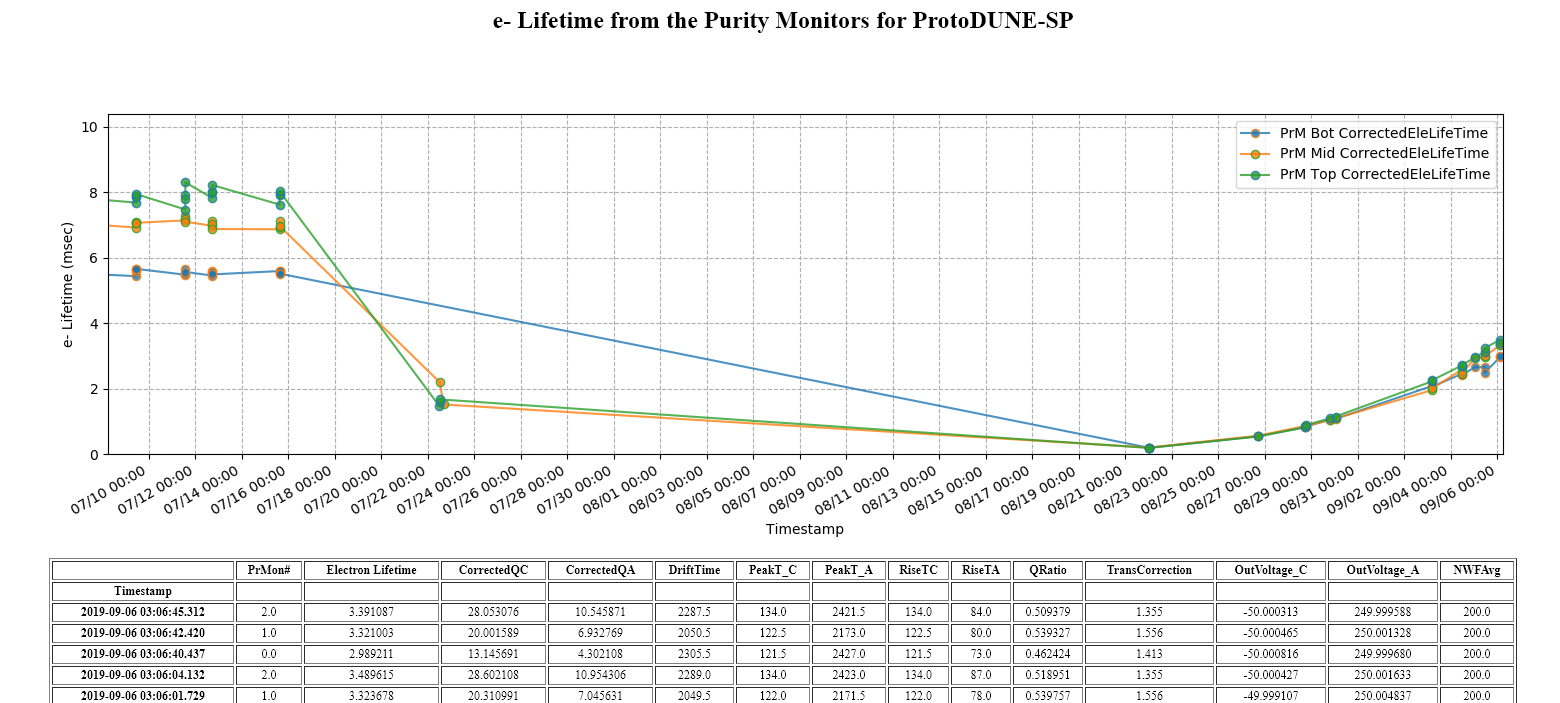
\includegraphics[width=1cm,clip]{figures/dqm_purmon_20190910_1.png}
\caption{Please write your figure caption here}
\label{fig-1}       % Give a unique label
\end{figure}

For two-column wide figures use syntax of figure~\ref{fig-2}
\begin{figure*}
\centering
% Use the relevant command for your figure-insertion program
% to insert the figure file. See example above.
% If not, use
\vspace*{5cm}       % Give the correct figure height in cm
\caption{Please write your figure caption here}
\label{fig-2}       % Give a unique label
\end{figure*}

For figure with sidecaption legend use syntax of figure
\begin{figure}
% Use the relevant command for your figure-insertion program
% to insert the figure file.
\centering
\sidecaption
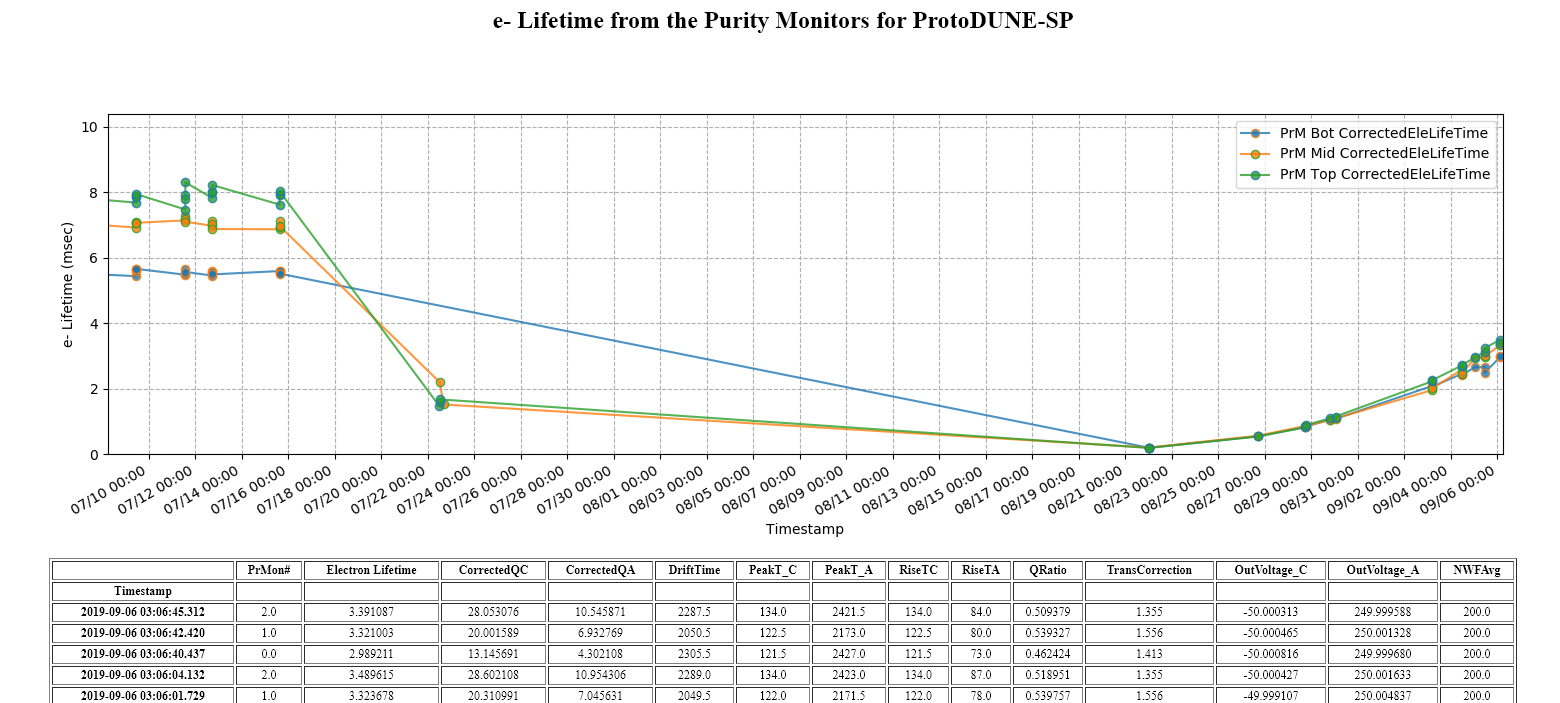
\includegraphics[width=5cm,clip]{figures/dqm_purmon_20190910_1.png}
\caption{Please write your figure caption here}
\label{fig-3}       % Give a unique label
\end{figure}

For tables use syntax in table~\ref{tab-1}.
\begin{table}
\centering
\caption{Please write your table caption here}
\label{tab-1}       % Give a unique label
% For LaTeX tables you can use
\begin{tabular}{lll}
\hline
first & second & third  \\\hline
number & number & number \\
number & number & number \\\hline
\end{tabular}
% Or use
\vspace*{5cm}  % with the correct table height
\end{table}

\begin{thebibliography}{99}

\bibitem{spanu}
M. Spanu
\emph{The status and results from ProtoDUNE Single Phase}
IOP Conf. Series: Journal of Physics: Conf. Series \textbf{1312} (2019) 012003

\bibitem{cdrVol1}
R. Acciarri et al.
\emph{Long-Baseline Neutrino Facility (LBNF) and Deep Underground Neutrino Experiment (DUNE) Conceptual Design Report Volume 1: The LBNF and DUNE Projects}.\\ ~e-Print: arXiv:\textbf{1601.05471}


\bibitem{cdrVol4}
R. Acciarri et al.
\emph{Long-Baseline Neutrino Facility (LBNF) and Deep Underground Neutrino Experiment (DUNE) Conceptual Design Report, Volume 4: The DUNE Detectors at LBNF}.\\~e-Print: arXiv:\textbf{1601.02984}

\bibitem{eps} M.Potekhin et al. \emph{The protoDUNE-SP experiment and its prompt
processing system}. Proceedings of Science (EPS-HEP2017) 513

\bibitem{chep18} M.Potekhin et al. \emph{The Prompt Processing System
and Data Quality Monitoring in the protoDUNE-SP Experiment}
EPJ Web of Conferences \textbf{214}, 01026 (2019)

\bibitem{django}
N. George \emph{Mastering Django: Core. The Complete Guide to Django 1.8 LTS}~ GNW Independent Publishing, ISBN: 099461683X

\bibitem{panda}
T. Maeno et al. \emph{Overview of ATLAS PanDA Workload Management.~J. Phys.: Conf. Series.} Vol.\textbf{331}. IOP Publishing, 2011,
doi:10.1088/1742-6596/331/7/072024


\bibitem{dirac}
A. Casajus et al.  \emph{DIRAC Pilot Framework and the DIRAC
Workload Management System.~J. Phys.: Conf. Series.} Vol.\textbf{219}. IOP Publishing, 2010,
doi:10.1088/1742-6596/219/6/062049

\bibitem{sam}
R. A. Illingworth \emph{A data handling system for modern and future Fermilab experiments.~J. Phys.: Conf. Series.} Vol.\textbf{513}. IOP Publishing, 2014,
doi:10.1088/1742-6596/513/3/032045

\bibitem{fts}
A. Norman \emph{The Fermilab File Transfer System}.~e-Print: FNAL CD-DocDB-5412

\bibitem{castoreos}
 L. Mascetti et al. \emph{Disk storage at CERN.~J. Phys.: Conf. Series.} Vol.\textbf{664}. IOP Publishing, 2015,
doi:10.1088/1742-6596/664/4/042035

\bibitem{eos_role}
S. Fuess et al. \emph{Design of the protoDUNE raw data management
infrastructure.~J. Phys.: Conf. Series.} Vol.\textbf{898}. IOP Publishing, 2017,
doi:10.1088/1742-6596/898/6/062036



\end{thebibliography}




\end{document}

% end of file template.tex

<div id='footer'><table width='100%'><tr><td class='right'><a href='http://fusioninventory.org/'><span class='copyright'>FusionInventory 9.1+1.0 | copyleft <img src='/glpi/plugins/fusioninventory/pics/copyleft.png'/>  2010-2016 by FusionInventory Team</span></a></td></tr></table></div>